\documentclass{article}

\usepackage{amsmath}
\usepackage{graphicx}

\newcommand{\rr}{\mathbf{r}}

\begin{document}

{\bf Quiz \#12; Tuesday, date: 04/17/2018}

{\bf MATH 53 Multivariable Calculus with Stankova}

{\bf Section \#114; time: 2 -- 3:30 pm}

{\bf GSI name: Kenneth Hung}

{\bf Student name:}

\vspace*{0.25in}

\begin{enumerate}
\item Use Green's Theorem to evaluate the line integral along the given positively oriented curve.
\[
\int_C \frac{1}{4} y^4 x \,dx + \frac{5}{2}y^3 x^2 \,dy,
\]
where $C$ is the circle $x^2 + y^2 = 4$.

\item {\em True / False?} Fix two points $A$ and $B$ in a simply connected domain $D$. If $\int_C \mathbf{F} \cdot d\rr$ is the same for all paths $C$ from $A$ to $B$, then $\mathbf{F}$ must be conservative on $D$.

\item {\em True / False?} Suppose $P$ and $Q$ has continuous partial derivatives everywhere. Green's Theorem cannot help us in computing line integral $\int_C \mathbf{F} \cdot d\rr$ where $C$ is given below.
\begin{center}
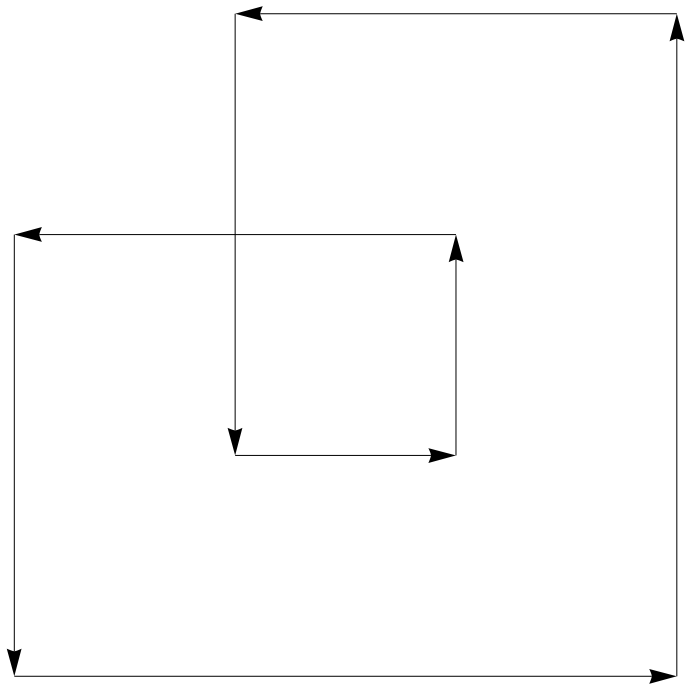
\includegraphics[width=0.33\textwidth]{quiz12dis114pic}
\end{center}
\end{enumerate}

\end{document}